\documentclass[12pt,margin=1in]{article}
\usepackage{lmodern}
\usepackage{amssymb,amsmath}
\usepackage{ifxetex,ifluatex}
\usepackage{fixltx2e} % provides \textsubscript
\ifnum 0\ifxetex 1\fi\ifluatex 1\fi=0 % if pdftex
  \usepackage[T1]{fontenc}
  \usepackage[utf8]{inputenc}
\else % if luatex or xelatex
  \ifxetex
    \usepackage{mathspec}
    \usepackage{xltxtra,xunicode}
  \else
    \usepackage{fontspec}
  \fi
  \defaultfontfeatures{Mapping=tex-text,Scale=MatchLowercase}
  \newcommand{\euro}{�}
\fi
% use upquote if available, for straight quotes in verbatim environments
\IfFileExists{upquote.sty}{\usepackage{upquote}}{}
% use microtype if available
\IfFileExists{microtype.sty}{%
\usepackage{microtype}
\UseMicrotypeSet[protrusion]{basicmath} % disable protrusion for tt fonts
}{}
\usepackage[margin=1in]{geometry}
\usepackage{graphicx}
\makeatletter
\def\maxwidth{\ifdim\Gin@nat@width>\linewidth\linewidth\else\Gin@nat@width\fi}
\def\maxheight{\ifdim\Gin@nat@height>\textheight\textheight\else\Gin@nat@height\fi}
\makeatother
% Scale images if necessary, so that they will not overflow the page
% margins by default, and it is still possible to overwrite the defaults
% using explicit options in \includegraphics[width, height, ...]{}
\setkeys{Gin}{width=\maxwidth,height=\maxheight,keepaspectratio}
\ifxetex
  \usepackage[setpagesize=false, % page size defined by xetex
              unicode=false, % unicode breaks when used with xetex
              xetex]{hyperref}
\else
  \usepackage[unicode=true]{hyperref}
\fi
\hypersetup{breaklinks=true,
            bookmarks=true,
            pdfauthor={},
            pdftitle={Is the Tea Party Libertarian, Authoritarian, or Something Else?},
            colorlinks=true,
            citecolor=black,
            urlcolor=red,
            linkcolor=black,
            pdfborder={0 0 0}}
\urlstyle{same}  % don't use monospace font for urls
\setlength{\parindent}{0pt}
\setlength{\parskip}{6pt plus 2pt minus 1pt}
\setlength{\emergencystretch}{3em}  % prevent overfull lines
\setcounter{secnumdepth}{0}

%%% Change title format to be more compact
\usepackage{titling}
\setlength{\droptitle}{-.25em}
  \title{Is the Tea Party Libertarian, Authoritarian, or Something Else?
\vspace{.25em}}
  \pretitle{\vspace{\droptitle}\centering\huge}
  \posttitle{\par}
  \author{}
  \preauthor{}\postauthor{}
  \date{}
  \predate{}\postdate{}


\usepackage{setspace}


\begin{document}


\begin{center}
Is the Tea Party Libertarian, Authoritarian, or Something Else?
\end{center}

\doublespacing

Scholars have been fascinated by the Tea Party since it first emerged on
the American political scene in the spring of 2009. While some have
dismissed it as simply a repackaging of conventional American
conservative populism, many have been struck by how effective it has
been in remobilizing the Republican Party base in the wake of the
Democratic electoral landslide of 2008. Most of the scholarship has
focused upon the demographic make up of its members (Courser 2012; Disch
2011; Maxwell and Parent 2012; Williamson, Skocpol, and Coggin 2011),
how it combines elements of elite and grassroots political mobilization
in new and innovative ways (Bailey, Mummolo, and Noel 2012; Karpowitz et
al. 2011), how it is a racialized response to the election of the first
African American President (Abramowitz 2012; Bailey, Mummolo, and Noel
2012; Disch 2011; Lowndes 2012; Skocpol and Williamson 2012) and how it
might connect with more militarized elements of the American far right
(Parker and Barreto 2013; Skocpol and Williamson 2012). Less attention
has been paid to the question of whether or not a specific ideology
might be driving support for the Tea Party. When ideology is explicitly
addressed, authors tend to note a peculiar contradiction in core beliefs
of Tea Party supporters: the Tea Party seems to embody an odd fusion of
libertarianism and social conservatism (Arceneaux and Nicholson 2012;
Berlet 2012; Montgomery 2012; Parker and Barreto 2013; Williamson,
Skocpol, and Coggin 2011; Wilson and Burack 2012). While we agree with
previous scholars who observe that the Tea Party does not have one
unifying ideology, we believe that political scientists have so far
underestimated or incompletely specified the unique ideological drivers
of Tea Party support.

The central claim of this article is that a crucial ideological factor
explaining support for the Tea Party is what Friedrich Nietzsche called
``misarchism'' in reference to the political philosophy of Herbert
Spencer. As we explain in detail below, distinct from both
libertarianism and social conservatism, misarchism refers to an aversion
to \emph{government} combined with support for the \emph{state} and
traditional morality. Consistent with the expectation of a misarchist
dimension in American attitudes, factor analysis on nine variables from
the 2012 American National Election Time-Series Study (ANES) reveals
that attitudes toward state power are positively intercorrelated with
attitudes toward traditional morality. Though neither are strongly
intercorrelated with attitudes toward government, the factor underlying
support for the state and traditional morality (which we call ``moral
statism'') is strongly and negatively correlated with the factor
underlying support for government. These results are consistent with the
Nietzschean diagnosis of misarchism as an ideological structure which
combines support for the state and moral traditionalism on a dimension which is
distinct from, and opposed to, attitudes toward government. Consistent
with the argument that misarchism is a crucial ideological driver of
support for the Tea Party, regression analyses reveal that the
interaction of moral statism with governmentalism (our
operationalization of misarchism) has, of all the independent variables
considered, one of the strongest and most robust partial correlations
with support for the Tea Party. Our findings have important
implications for our understanding of right-wing ideology in the United
States and they help to resolve the puzzle of the Tea Party's still
poorly understood and contradictory ideological components.

The article proceeds in five sections. The first section elaborates the
puzzle of the Tea Party's ideological composition. The second section
details the theory that misarchism is a key ideological component of Tea Party support,
which helps to explain the Tea Party's puzzling tendency to appear both libertarian and authoritarian. The
third section explains our research strategy, including a discussion of
our data and modeling approach. A fourth section presents the analysis
with a discussion of findings, and a fifth section concludes.

\textbf{Libertarians, Conservatives, or Something
Else?}

There are currently two dominant accounts of Tea Party ideology in the
academic literature. The first approach argues that Tea Party support is
driven largely by far right-wing support within the Republican Party
(Burack and Snyder-Hall 2012; Parker and Barreto 2013; Skocpol and
Williamson 2012). The second approach downplays the role of ideology by
contending that the Tea Party does not represent the ideology of members
but is rather a decentralized group of diverse viewpoints exploited by
party elites (Bailey, Mummolo, and Noel 2012; Karpowitz et al. 2011; Lo
2012; Williamson, Skocpol, and Coggin 2011). The first approach uses the
standard linear conceptualization of ideology as ranging from left to
right along a single dimension (Knight 2006, 619), whereas the second
approach denies that ideology has much of a role in explaining Tea Party
support. Contra the first account of the Tea Party, we think that the
specific ideology of ``misarchism'' can explain some important
differences between Tea Party members and other conservatives that is
not easily captured in the left-right conceptualization of ideology.
Contra the second account of the Tea Party, our argument is that
ideology can explain an important aspect of Tea Party support.

One prominent example of explaining Tea Party supporters as consisting
largely of the ``far right'' of the American political spectrum is the
detailed analysis of the Tea Party by Christopher S. Parker and Matt A.
Barreto. They argue that the Tea Party is the latest manifestation of
``reactionary conservatism'' (Parker and Barreto 2013; Robin 2013). They
describe reactionary conservatives as individuals on the far right of
the political spectrum who participate in a ``paranoid style'' of
politics that sees ``others'' as a threat to the traditional vision of
America. They locate the Tea Party as inheritors of the political
tradition of the John Birch society and the KKK (Parker and Barreto 2013, 35).
According to Parker and Barreto, the election of the USA's first African-American President
mobilized this reactionary strand of conservatism and drove support for
the Tea Party. While there are other examples, the Parker and Barreto
version of Tea Party ideology is emblematic because it considers
ideology in a traditional one-dimensional, left-right spectrum. The
party can be labeled ``reactionary'' because it is further to the right
on the ideological spectrum than ``mainstream'' conservatism (Parker and
Barreto 2013, 48).

The left-right ideological spectrum approach, however, has a difficult
time explaining Tea Party support (Carmines and D'Amico 2014, 214).
Scholars will observe that the movement seems to combine elements of
libertarianism and social conservatism (Wilson and Burack 2012; Parker and Barreto 2013, 174;
Arceneaux and Nicholson 2012, 701; Skocpol and Williamson 2012,
35). All of these different accounts of the Tea Party struggle with
the apparent puzzle of how the Tea Party reconciles its apparently
contradictory commitments to smaller government on the one hand, and
calls for greater government intervention in areas such as morality and
immigration on the other hand.

This synthesis can lead to some apparent contradictions in policy
preferences. First, the Tea Party members (at least in public opinion
polling) seem to favour existing entitlement programs such as Social
Security and Medicare while opposing other programs such as Temporary
Assistance for Needy Families (TANF) and the Affordable Care Act
(Skocpol and Williamson 2012, 54--68). Second, Tea Party members are
quite concerned about government intervention with respect to firearms,
but are strongly in favour of increased intervention in terms of
immigration enforcement and counter-terrorism (Parker and Barreto 2013,
165--72; Skocpol and Williamson 2012, 71--72). Third, while the Tea
Party expresses deep concern about government programs aimed at trying
to alter the behavior of citizens (such as Michelle Obama's anti-obesity
campaign) they also express a general concern that America's moral
collapse is at the root of most contemporary problems (Jones, Cox, and
Navarro-Rivera 2013; McCalmont 2013). We will contend that these
apparent contradictions about Tea Party supporters' policy preferences
make more sense if we view them as expressions of an underlying
misarchist ideology.

\textbf{A Theory of the Tea Party as a Misarchist
Movement}\label{a-theory-of-the-tea-party-as-a-misarchist-movement}

By ideology we mean ``a
set of ideas, beliefs, opinions and values that: 1) exhibit a recurring
pattern, 2) are held by significant groups, 3) compete over providing
and controlling plans for public policy, and 4) do so with the aim of
justifying, contesting or changing the social policy and political
arrangements and processes of a political community'' (Freeden 2003,
100). Existing research on the Tea Party has downplayed the ideological
dimension. Parker and Barreto in their research control for ideology as
one possible factor in Tea Party support and find that it is not
statistically significant (Parker and Barreto 2013, 100). Others have
argued that the Tea Party does not have a coherent ideology. Instead it
is more a product of top-down organization via well-funded PACs, wealthy
individuals such as the Koch brothers, and media support through venues
such as Fox News (Lo 2012).

One reason most scholars of the Tea Party neglect the possibility of an
ideological basis for Tea Party support is the influential current of
scholarship which suggests the general public is not characterized by
coherent belief systems (Campbell et al. 1960; Converse 1964; Lewis-Beck
et al. 2008). An overarching argument in this current is that most
citizens' attitudes do not reflect enough information, stability, or
consistency to be considered ideological. Given such findings, how could
a certain ideology help to explain Tea Party support? A burgeoning
research agenda in political psychology suggests that political
attitudes are indeed characterized by substantial, underlying
psychological differences which correlate with ideological
self-placement (Goren 2013; Graham, Haidt, and Nosek 2009; Haidt 2012).
Haidt argues that the difference between liberals, conservatives and
libertarians in the U.S. is that their moral systems are based on
different psychological foundations (Graham, Haidt, and Nosek 2009;
Haidt 2012). In a similar vein, Goren demonstrates that voters do not
vote on liberal-conservative predispositions but rather genuine policy
principles, namely, limited government, traditional morality, and
military strength (Goren 2013). Our argument is that misarchism is a
particular combination of precisely such policy principles, a
combination which represents a unique source of Tea Party support and is
distinct from other ideological currents prominent on the contemporary
American right, namely conventional conservatism and libertarianism.

Nietzsche used the term misarchism as a pejorative term to describe the
biological and political philosophy of Herbert Spencer (Nietzsche 2007,
52). He argued that at the core of Spencer's philosophy was a hatred of
rule (as the term misarchy comes from the Greek roots \emph{misein} for
hatred and \emph{archos} for ruler). Spencer hated the government,
because government polices and regulations limited human freedom.
Spencer believed that the government's practice of conducting the
conduct of individuals would short-circuit the development of his end
goal for society: an individual who would be completely self-reliant and
altruistic. Government policies interfered with the evolutionary
process, and enabled less fit, or unfit individuals to survive.
According to Spencer this was a threat to the overall strength and
health of a society. The government was bad not simply because it
limited negative liberty; it was bad because it threatened the full
development of the species. A society without government would enable
human evolution in both physiological and moral terms. Humans would have
a longer life expectancy, would be stronger, and would develop morally
in a way in which they reconciled altruistic and egoistic impulses.
Eventually a fully morally-evolved person would selfishly pursue ends
that were for the benefit of society as a whole. He labeled this type of
person the ``ideally moral man'' (Spencer 1879, 75).

Critics of Spencer, including Thomas Huxley and
Nietzsche, noticed a peculiar feature of Spencer's political philosophy:
he was opposed to any use of the government to redistribute wealth,
alleviate poverty, to regulate professions such as health care, to fund
and regulate a public education system, or to spend on infrastructure,
yet he was strongly supportive of the state increasing its policing
power to maintain order. In his rejoinder to Spencer, Huxley labeled the
political philosophy alternately ``administrative nihilism'' and
``astynomocracy'' (police government) (Huxley 1871). While Spencer's
vision of a minimalist state appeared to promote human freedom, he had
developed a model that eliminated all the regular administrative
activities that a government engages in and replaced it with a state
that was fully vested in its police powers.

The terms government and state are often used
interchangeably but in order to understand how misarchism works as an
ideology, we need to differentiate these two terms. We follow Max Weber
in defining the state as the ``monopoly on legitimate physical
violence'' (Weber 2004, 33). We follow Michel Foucault in defining
government as the ``\,`the conduct of conduct': a form of activity
aiming to shape, guide or affect the conduct of some person or persons''
(Foucault 1991; Gordon 1991, 2). The state uses its monopoly on violence
to dominate its subjects and punish violations of the law. Conversely
government uses techniques such as education, regulation,
administration, and management to shape human behaviour. While states
have governments, government is not limited to the state. For instance,
both for-profit and non-profit corporations have boards of governors and
business schools teach corporate governance.\footnote{Political theorist
  John Hoffman (1995) draws a similar distinction between statism and
  governmentalism, where the state refers to the use of force to tackle
  conflict and the government refers to the use of negotiation and
  arbitration to resolve conflicts of interest.}

Our point is that one can be anti-government while being pro-state. If
this position seems odd it is only because we are seeking to identify an
ideology distinct from more established ideologies about government
authority. Classical libertarians are strongly skeptical of both state
power and government power. Libertarianism as an ideology holds that
individual freedom is the greatest good and favors policies that
maximizes individual freedom in both the economic and social sphere and
seeks to minimize government interference as much as possible (Brennan
2012, 1--3). There are crucial differences in policy preferences between
Tea Party supporters and Libertarians on issues such as NSA
surveillance, the use of drone warfare, aggressive U.S. foreign policy,
and the continuation of the war on drugs. Libertarians tend to oppose
state power in these areas, whereas Tea Party members are more likely to
be supportive of increasing state power in these domains. All these
programs involve increasing the state's use of the instruments of
violence in order to counter perceived threats to the state. Where
libertarians and misarchists agree is on their opposition to
governmentalism; to using government programs and policies to shape the
behaviour of individuals, and to improve the well-being of society.
Traditional conservatives tend to be skeptical of both state power and
governmental power but are more moderate. Conservatism is an ideology
that defends preservation of the status quo and values traditional
social and political structures, preferring incremental social change to
more radical proposals for reform or revolution (Heywood 2007, 65).
Traditional conservatives recognize the need for some statism and some
governmentalism, but are also skeptical of the extremism of both
libertarians and misarchists, who favour the abolition of almost all
government (in both cases) and the minimization of the state (in the
case of libertarians).

Based on this reading of Nietzsche, we define misarchism as an
ideological constellation which combines three general attitudes. It
combines attitudes which are 1) anti-government, 2) pro-state, and 3)
moralistic. Anti-government attitudes are those which reflect opposition
to using government policy to improve the condition and behaviour of
individuals and society in general. Misarchists will oppose wealth
redistribution and any programs that aim at assisting individuals in
need. They will also oppose government attempts to regulate individual
behaviour. Pro-state attitudes reflect support for the state using its
monopoly on violence to maintain order and confront perceived threats to
society. Moralistic attitudes are those which see the cultivation of
individual morality rather than government regulation as the best way to
promote a good society.

Finally, Nietzsche's diagnosis of misarchism as an ideology is
surprisingly consistent with certain findings in contemporary empirical
research. In particular, Goren finds that citizens have genuine policy
principles which they rely on for presidential vote choice. He
identifies three core ``policy principle cleavages:'' limited
government, traditional morality, and military strength. While Goren
does not investigate Nietzsche's argument about the specific misarchist
combination of these factors, Goren's findings increase the plausibility
of our argument--which we arrived at independently through Nietzsche and
Spencer--that a particular combination(s) of precisely these factors can
help to explain the Tea Party's ideological composition and at least one
key source of its support.

\textbf{Research Design}\label{research-design}

To test our argument, we examine data from the 2012 ANES. We selected
the 2012 ANES because it is the largest and most recent survey of
Americans to measure the wide variety of social and political attitudes
required to test our hypotheses.\footnote{The Cooperative Congressional
  Election Survey, used in some previous research on the sources of Tea
  Party support (Bradberry and Jacobson 2014), has a much larger sample
  than the ANES but does not include direct measures of moral
  traditionalism.} Specifically, to investigate the existence and
potential structure of misarchism, we select a total of nine variables,
three variables gauging each of the ideological strands discussed above
(moral traditionalism, governmentalism, and statism.) First, three
variables measure attitudes toward government activity related to
policing power. The variable \emph{Defense} measures on a seven point
scale how much the respondent thinks should be spent on defense.
\emph{Immigration} measures respondent support for laws allowing
immigration status checks on suspects, measured on a three point scale
reflecting opposition, neither opposition nor support, and support.
\emph{Wiretapping} measure support for government wiretapping powers on
a three point scale, reflecting whether respondents think such powers
``have gone too far'', ``are just about right'', or ``do no go far
enough.'' Three variables measure attitudes toward government
interventions not related to policing power. \emph{Jobs} measures on a
seven point scale how much the respondent supports the government
guaranteeing jobs or income. \emph{Services} measures on a seven point
scale support for government provision of services. \emph{Guns} measures
on a seven point scale support for federal laws which make it harder to
purchase a gun. Three variables capture moral conservatism.
\emph{Morals} measures on a 5-point Likert scale disagreement with the
statement, ``The world is always changing and we should adjust our view
of moral behavior to those changes.'' \emph{Intolerant} measures on a
5-point Likert scale disagreement with the statement, `We should be more
tolerant of people who choose to live according to their own moral
standards, even if they are very different from our own.' \emph{Family}
measures on a 5-point Likert scale agreement with the statement, ``This
country would have many fewer problems if there were more emphasis on
traditional family ties.'' Lastly, we include in the factor analysis a
measure of left-right ideology, \emph{Conservatism}, using respondent
self-placement on the conventional 7-point liberal-conservative
scale.\footnote{We do not include any measure of racial animosity
  because the experiment conducted by Arceneaux and Nicholson produces
  little evidence that racial animosity is independently associated with
  Tea Party support, even though Tea Party supporters appear more likely
  to oppose government benefits due to racial resentment.}

Analysis proceeds in two stages. In a first stage, we employ exploratory
factor analysis to explore whether a smaller set of latent variables
underlies the nine original variables in some fashion consistent with
the notion of misarchism. If our argument is correct, factor analysis should reveal that attitudes
toward government, the state, and moral traditionalism are characterized
by some structure of non-trivial inter-correlation consistent with Nietzsche's diagnosis. We would then
extract for each respondent their score for each factor, allowing us to
assign each individual a value on each of the latent ideological
variables which structure these attitudes.

In a second stage, we test whether the latent ideological dimensions
identified in the factor analysis help to explain support for the Tea
Party. If our argument is correct, we expect that latent ideological
dimension(s) approximating what we call misarchism should be positively
associated with Tea Party support. We estimate a series of logistic
regressions on the dependent variable \emph{Support}, which is a binary
variable taking the value of one for all respondents who say they
support the Tea Party and a zero for all who oppose or neither support
nor oppose. In this stage of analysis, the key independent variables are
the latent variables extracted from the factor analysis. We also include
a variety of standard control variables drawn from previous research.
First, we include a battery of standard variables commonly found to be
associated with political attitudes, including \emph{Race} (white or
non-white), \emph{Gender} (male or female), \emph{Age}, \emph{Income},
(28 ordinal categories we convert to a numerical variable),
\emph{Education} (16 ordinal categories we use as a numerical variable),
and \emph{Religion} (a dummy variable for those who attend religious
services). \emph{PartyID} is a 7-point ordinal scale we convert to a
numerical scale in which the lowest values represents strong
identification with the Democratic Party and the highest value
represents strong identification with the Republican Party. To control
for the argument that a unique driver of Tea Party support is aversion
to Barack Obama (Bradberry and Jacobson 2014; Maxwell and Parent 2012;
Parker and Barreto 2013), we include the ``feeling thermometer'' measure
of feelings toward the 2012 Democratic Presidential candidate on a
100-point scale. We also control for authoritarianism (Arceneaux and
Nicholson 2012, 701) with a variable of that name. Specifically, we take
the mean value of four responses to questions about the most important
traits in a child, where the authoritarian value is assigned a value of
1 and the other a value of 0: ``obedience'' or ``self-reliance,''
``respect for elders'' or ``independence,'' ``good manners'' or
``curiosity,'' and ``well behaved'' or ``considerate.'' To control for
evangelicalism, which previous studies have found to be associated with
Tea Party support (Arceneaux and Nicholson 2012; Bradberry and Jacobson
2014; Maxwell and Parent 2012; Parker and Barreto 2013), we include the
variable \emph{BornAgain}, which takes a value of 1 for respondents who
have had a personal conversion experience related to Jesus Christ and 0
otherwise. Finally, we control for the possible effect of watching the
Fox News Channel, which Parker and Baretto find to be a significant
predictor of Tea Party support after controlling for attitudes toward
Obama and a wide variety of other factors. The variable \emph{FoxNews}
takes a value of 1 for all respondents who report watching any of a
series of Fox News programs listed by the ANES.\footnote{These include
  the programs \emph{Fox Report}, \emph{The Five}, \emph{America's
  Newsroom,} as well as the eponymous programs featuring Greta Van
  Susteren, Sean Hannity, Mike Huckabee, Brett Baier, and Bill O'Reilly.}

\textbf{Analysis}\label{analysis}

First, we report results from a factor analysis using the extraction
method of maximum likelihood and an oblique rotation. Additional technical information, numerical results, and diagnostics for the factor analysis can be found in Supplementary Information. Results of the
factor analysis are broadly consistent with our argument; attitudes toward
policing powers correlate positively with moral traditionalism, in a way
distinct from any possible correlation between moral traditionalism and
governmentalism. Figure 1 plots the factor loadings of our nine
attitudinal variables, with axes labeled to reflect our interpretation
of the
factors.\footnote{To improve readability, abbreviated variable names and a random jitter of .3 was applied to the width and height of each point on the plot.}
In Figure 1, the horizontal location of a variable reflects the degree
to which it loads onto the latent variable we call moral statism, while
the vertical location reflects the degree to which it loads onto the
latent variable we call governmentalism.

As Figure 1 reveals, attitudes toward policing powers as well as morally
traditional attitudes are correlated with Factor 1 (clustered in the
bottom-right). Attitudes toward traditional government interventions in
society are positively correlated with Factor 2. Factor 1, which appears
to capture a moral-statist dimension in public attitudes, explains 17\%
of the overall variance while Factor 2, reflecting governmentalism,
explains 15\%. \emph{Morals}, \emph{Immigration}, and
\emph{Conservatism} are only weakly negatively correlated with
governmentalism, while the governemntalist attitudes are not positively
or negatively correlated with moral statism to any significant degree.
The key implication of the factor analysis is that moral traditionalism
and policing powers are correlated along a dimension irreducible to
anti-govermentalism, suggesting that the conventional wisdom about the
ideology of libertarianism incorrectly conflates two distinct
ideological patterns.

\begin{center}
[Figure 1 about here]
\end{center}

It is important to note that we should not expect adequate overall model
fit, for two reasons. First, we are not arguing our hypothesized latent
factors should explain so much of the variation in these nine variables
as to be a fully adequate model of them. We are only arguing that these
nine variables should contain certain identifiable, non-trivial latent
factors a combination of which will explain a unique portion of Tea
Party support. Second, the survey questions refer to diverse political
phenomena and likely reflect a great deal of variation admittedly
irreducible to our hypothesized factors. Given our research interests,
at this stage, it is adequately consistent with our theory to observe
that the first two factors identified by the factor model capture latent
dimensions reflective of our expectations.

Do the latent ideological variables of governmentalism and moral statism
help improve our understanding of support for the Tea Party? Table 1
shows results from two logistic regressions modeling the probability
that an individual will support the Tea Party. Before analysis, each
independent variable was centered to a mean of zero and divided by two
standard deviations, including the factor scores, so that all
coefficients can be interpreted as the expected change in the log-odds
of supporting the Tea Party associated with a two-standard-deviation
change in the independent variable (or a one-category change in the case
of a categorical variable). Model 1 is a baseline model including
predictors from previous research and standard demographic control
variables. Model 2 adds each of the latent variables and a term
representing the multiplicative interaction of the two. Model 2 does not
include \emph{Conservatism} because it was included in the factor
analysis and would therefore be redundant.\footnote{It may be objected
  that to fully test our argument that misarchist ideology explains a
  unique portion of Tea Party support, we would have to do so
  controlling for liberal-conservative self-placement. We therefore run
  a separate model similar to Model 2 but including \emph{Conservatism}
  as a covariate (see Supplementary Information). \emph{Conservatism} is
  positive and statistically significant and the estimates for
  \emph{Government} and the interaction term remain substantially the
  same as in Model 2. \emph{MoralStatism} is no longer statistically
  significant but has a variance inflation factor of 4.259 suggesting
  collinearity likely due to the redundancy of \emph{Conservatism}.}
  
 \begin{center}
[Table 1 about here]
\end{center}

Given a typical respondent who hypothetically changes from the 10th percentile
of moral statism to the 90th when governmentalism is equal to zero, we
would expect the probability of them supporting the Tea Party to
increase by 6\% (sd = 2), from 0.04 to 0.1 on average.\footnote{All discussion of effect sizes refer to
 1000 simulations of Model 2 in Table 1, generated using the R package \emph{Zelig} (Imai, King, and Lau 2009).} Given a typical
respondent who hypothetically changes from the 90th percentile of
governmentalism to the 10th when moral statism is equal to zero, we
would expect the probability of them supporting the Tea Party to
increase by 7\% (sd = 3), from 0.04 to 0.11 on average. To gain a sense
of how much governmentalism conditions the effect of moral statism is
somewhat more complicated. The coefficient in Model 2 for
\emph{MoralStatism:Government} reflects the estimated effect that a
two-standard-deviation increase in governmentalism has on the estimated
effect a two-standard-deviation increase in moral statism would have on
the log-odds of someone supporting the Tea Party. Because a substantive
interpretation of this interactive effect requires us to consider
multiple values for both variables all at once, Figure 2 plots the
expected effect of moral statism across its range for three different
values of governmentalism (the 10th, 50th, and 90th percentiles). Figure
2 reveals strikingly how high the expected probability of supporting the
Tea Party reaches when individuals' ideological perspective is
characterized by strong moral statism and strong anti-governmentalism.
Individuals characterized by the highest observed levels of moral
statism also in the 90th percentile of anti-governmentalism (below a
value of -.7 on the governmentalism factor) have a probability of
supporting the Tea Party around 40\%. To be more precise, moving from
minimum to maxium moral statism while in the 10th percentile of
governmentalism increases the probability of supporting the Tea Party by
.39 (sd=.07) more than it would in the 90th percentile of
govermentalism, from .01 (sd=.00) to .42, (sd=.07) rather than .05
(sd=.02) to .03 (sd=.02).


\begin{center}
[Figure 2 about here]
\end{center}

Does the misarchist interaction of moral statism and
anti-governmentalism also drive Republican Party identification and/or
conservative identification? The answer matters for understanding how
these model results improve our understanding of American conservatism.
If a misarchist perspective is associated with Republican Party
identification or identification with conservatism in general, our
findings may only reflect a substrate of American conservatism but not
necessarily Tea Party support per se. To check this possibility, we run
two additional models similar to Model 2 but using ordinary least
squares estimation with \emph{PartyID} and \emph{Conservatism} on the
left-hand side of the model equation instead of the right-hand side. To
save space, we provide only a brief discussion of the results here, with
full model results available in the Supplementary Information. Moral
statism positively predicts and governmentalism negatively predicts
Republican identification with high levels of statistical significance,
but the coefficient for the interaction term is nearly zero and
statistically insignificant. On the other hand, considering conservative
self-identification as the dependent variable, while both moral statism
and governmentalism are again signed as expected, the interaction term
is positive and significant. These results suggest that the misarchist
interaction of moral statism and anti-governmentalism is positively
associated with Tea Party support in a fashion irreducible to simple
Republican Party identification or conservative identification. A
substantive interpretation consistent with these auxiliary models is
that the Republican Party is home to morally statist as well as
anti-government and pro-government attitudes (a ``broad church''
encompassing various forms of conservatism). On the other hand, the Tea
Party is uniquely associated with the combination of morally statist and
anti-government attitudes whereas simple ``conservatism'' is uniquely
associated with morally statist and pro-government attitudes. Because
these are not our primary, theoretically motivated arguments, caution
should be exercised in making inferences from these auxilliary models.
Nonetheless, they strengthen support for our argument and contradict the
common interpretation of Tea Party supporters as simply extreme
conservatives or extreme Republicans.

To check the robustness of our results, we also executed a series of
additional analyses. The full results from these analyses, with
additional detail on the procedures and discussion of the results, can
be found in Supplementary Information. In short, we consider three main
threats to regression-based inferences from observational data. First,
to guard against parametric model dependence, we use a genetic matching
algorithm to identify that subset of the original dataset for which the
distribution of each covariate is optimally balanced across both
treatment and control groups (Diamond and Sekhon 2012).
From this subset of matched pairs we estimate an average treatment
effect for those ``treated'' to the misarchist interaction. Second,
because we do not know the true model, an idiosyncratic search for
optimal model specifications can lead to bias (Montgomery and
Nyhan 2010, 4). To gauge the sensitivity of our results to model
selection, we use Bayesian Model Averaging (BMA) to calculate posterior
probabilities for all possible coefficients and models in order to
identify the most likely models and variables. Finally, another possible
problem is that listwise deletion of all observations containing missing
values may have led to biased estimates. To consider this, we employ
multiple imputation of missing values and re-estimate the regression
models. While all of these robustness checks provide additional
information and important nuance for evaluating our main argument,
overall they suggest the conclusions we have drawn here are not merely
artifacts of parametric model dependence, arbitrary model selection, or
missing data, respectively.

\textbf{Conclusion}\label{conclusion}

This article demonstrates that an ideological constellation first
diagnosed by Nietzsche as ``misarchism''---a combination of
anti-government, pro-state, and moralistic attitudes---helps to predict
Tea Party support and generally improves our understanding of the
ideological nature of the Tea Party movement. In particular, we leverage
the history of political theory to provide a coherent solution to the
otherwise inexplicable combination of libertarianism and
authoritarianism which scholars have found to co-exist within the Tea
Party. While we find additional support for some previous
findings---namely, that feelings toward Obama, evangelicalism, and
exposure to Fox News are significant and robust predictors of Tea Party
support---this article is the first to provide systematic empirical
evidence that a particular ideological constellation irreducible to
libertarianism or social conservatism is a unique and notably strong
driver of Tea Party support.

Our ideological explanation also raises an interesting question about
the future of the Tea Party. If opposition to Obama were the primary
driver of Tea Party support, then we would expect Tea Party mobilization
to subside once Obama's term as President ends. If however, a
significant driver of Tea Party mobilization is a misarchist ideology,
then we would expect the Tea Party to continue to play a role in the
Republican party by supporting candidates and policies that would be in
line with misarchist beliefs long after President Obama leaves office.

There are several questions about misarchism that this study does not
answer, but are worthy of further investigation. The first is whether
misarchism represents a new ideology within the Republican party, or if
it is an ideology that has somehow been a latent feature of American
political life. If it is new, then this would raise some interesting
questions about how new ideologies form. Did the election of Obama, or a
backlash against the Stimulus Act and the Affordable Care Act, somehow
crystallize a new constellation of beliefs in the minds of a large bloc
of voters? Alternatively, was this a latent worldview held by a large
segment of the electorate that was somehow mobilized through and elite
branding campaign by Conservative activist groups such as FreedomWorks
and media outlets such as Fox News? More generally, our approach, by
thinking about the possibility of unique and diverse ideological
constellations structuring attitudes within the conventional left-right
spectrum, raises questions about what other ideological constellations
may mobilize different constituencies in American politics.

\pagebreak

\textbf{References}\label{references}

\setlength{\parindent}{-0.2in} \setlength{\leftskip}{0.2in}
\setlength{\parskip}{8pt} \vspace*{-0.2in} \noindent

Abramowitz, Alan I. 2012. ``Grand Old Tea Party: Partisan Polarization
and the Rise of the Tea Party Movement.'' In \emph{Steep: The
Precipitous Rise of the Tea Party}, Berkeley, California: University of
California Press, 195--211.

Arceneaux, Kevin, and Stephen P. Nicholson. 2012. ``Who Wants to Have a
Tea Party? The Who, What, and Why of the Tea Party Movement.'' \emph{PS:
Political Science \& Politics} 45(04): 700--710.

Bailey, Michael A., Jonathan Mummolo, and Hans Noel. 2012. ``Tea Party
Influence: A Story of Activists and Elites.'' \emph{American Politics
Research} 40(5): 769--804.

Berlet, Chip. 2012. ``Reframing Populist Resentments in the Tea Party
Movement.'' In \emph{Steep: The Precipitous Rise of the Tea Party}, eds.
Christine Trost and Lawrence Rosenthal. Berkeley, California: University
of California Press, 42--66.

Bradberry, Leigh A, and Gary C Jacobson. 2014. ``The Tea Party and the
2012 presidential election.'' \emph{Electoral Studies}.
\href{Online only: http://bit.ly/1DsIbv9}{Online only: http://bit.ly/1DsIbv9}.

Brennan, Jason. 2012. \emph{Libertarianism: What Everyone Should Know}.
Oxford: Oxford University Press.

Burack, Cynthia, and R. Claire Snyder-Hall. 2012. ``Introduction:
Right-Wing Populism and the Media.'' \emph{New Political Science} 34(4):
439--54.

Campbell, Angus, Philip E Converse, Warren E Miller, and Donald E
Stokes. 1960. \emph{The American Voter}. Chicago: University of Chicago
Press.

Carmines, Edward G, and Nicholas J D'Amico. 2014. ``The New Look in
Political Ideology Research.'' \emph{Annual Review of Political Science}
18(1): 205--16.

Converse, Philip E. 1964. ``The Nature of Belief Systems in Mass
Publics.'' In \emph{Ideology and Its Discontents}, ed. David E Apter.
New York: The Free Press of Glencoe.

Courser, Zachary. 2012. ``The Tea `Party' as a Conservative Social
Movement.'' \emph{Society} 49(1): 43--53.

Diamond, Alexis, and Jasjeet S Sekhon. 2012. ``Genetic Matching for
Estimating Causal Effects: A General Multivariate Matching Method for
Achieving Balance in Observational Studies.'' \emph{Review of Economics
and Statistics} 95(3): 932--45.

Disch, Lisa. 2011. ``Tea Party Movement: The American `Precariat'?''
\emph{Representation} 47(2): 123--35.

Foucault, Michel. 1991. ``Governmentality.'' In \emph{The Foucault
Effect: Studies in Governmentality}, eds. Graham Burchell, Colin Gordon,
and Peter Miller. Chicago: University of Chicago Press, 87--104.

Freeden, Michael. 2003. \emph{Ideology: A Very Short Introduction}.
Oxford: Oxford University Press.

Gordon, Colin. 1991. ``Governmental Rationality: An Introduction.'' In
\emph{The Foucault Effect: Studies in Governmentality}, eds. Graham
Burchell, Colin Gordon, and Peter Miller. Chicago: University Of Chicago
Press, 1--52.

Goren, Paul. 2013. \emph{On Voter Competence}. Oxford: Oxford University
Press.

Graham, Jesse, Jonathan Haidt, and Brian A Nosek. 2009. ``Liberals and
conservatives rely on different sets of moral foundations.''
\emph{Journal of Personality and Social Psychology} 96(5): 1029--46.
\url{http://psycnet.apa.org/journals/psp/96/5/1029.html}.

Haidt, Jonathan. 2012. \emph{The Righteous Mind: Why Good People are
Divided by Politics and Religion}. New York: Pantheon.

Heywood, Andrew. 2007. \emph{Political Ideologies}. 4th ed. Basingstoke:
Palgrave Macmillan.

Hoffman, John. 1995. \emph{Beyond the State: An Essay in Interpretation:
An Introductory Critique}. Cambridge, UK: Polity Press.

Huxley, Thomas. 1871. ``Administrative Nihilism (1871).''
\url{http://aleph0.clarku.edu/huxley/CE1/AdNil.html} (April 12, 2014).

Imai, Kosuke, Gary King, and Olivia Lau. 2009. ``Zelig: Everyone's
Statistical Software.'' \url{http://gking.harvard.edu/zelig}.

Jones, Robert P, Daniel Cox, and Juhem Navarro-Rivera. 2013. ``2013
American Values Survey: In Search of Libertarians in America.''
\emph{Public Religion Research Institute}.
\url{http://publicreligion.org/research/2013/10/2013-american-values-survey/}
(September 18, 2014).

Karpowitz, Christopher F., J. Quin Monson, Kelly D. Patterson, and
Jeremy C. Pope. 2011. ``Tea Time in America? The Impact of the Tea Party
Movement on the 2010 Midterm Elections.'' \emph{PS: Political Science \&
Politics} 44(02): 303--9.

Knight, Kathleen. 2006. ``Transformations of the Concept of Ideology in
the Twentieth Century.'' \emph{American Political Science Review}
100(04): 619.

Lewis-Beck, Michael S, William G Jacoby, Helmut Norpoth, and Herbert F
Weisberg. 2008. \emph{The American Voter Revisited}. Ann Arbor:
University of Michigan Press.

Lo, Clarence Y. H. 2012. ``Astroturf Versus Grass Roots: Scenes from
Early Tea Party Mobilization.'' In \emph{Steep: The Precipitous Rise of
the Tea Party}, eds. Lawrence Rosenthal and Christine Trost. Berkeley,
California: University of California Press, 98--130.

Lowndes, Joseph. 2012. ``The Past and Future of Race in the Tea Party
Movement.'' In \emph{Steep: The Precipitous Rise of the Tea Party}, eds.
Christine Trost and Lawrence Rosenthal. Berkeley, California: University
of California Press, 152--70.

Maxwell, Angie, and T Wayne Parent. 2012. ``The Obama Trigger:
Presidential Approval and Tea Party Membership.'' \emph{Social Science
Quarterly} 93(5): 1384--1401.

McCalmont, Lucy. 2013. ``Poll: Most Libertarians Don't Identify as Tea
Partiers.'' \emph{POLITICO}. \url{http://politi.co/1Lr7tSe} (September
18, 2014).

Montgomery, Jacob M, and Brendan Nyhan. 2010. ``Bayesian Model
Averaging: Theoretical Developments and Practical Applications.''
\emph{Political Analysis} 18(2): 245--70.

Montgomery, Peter. 2012. ``The Tea Party and the Religious Right
Movements: Frenemies with Benefits.'' In \emph{Steep: The Precipitous
Rise of the Tea Party}, eds. Christine Trost and Lawrence Rosenthal.
Berkeley, California: University of California Press, 242--74.

Nietzsche, Friedrich Wilhelm. 2007. \emph{On the Genealogy of Morality}.
ed. Keith Ansell-Pearson. Cambridge, UK: Cambridge University Press.

Parker, Christopher S., and Matt A. Barreto. 2013. \emph{Change They
Can't Believe In: The Tea Party and Reactionary Politics in America}.
Princeton University Press.

Robin, Corey. 2013. \emph{The Reactionary Mind: Conservatism from Edmund
Burke to Sarah Palin}. New York: Oxford University Press USA.

Skocpol, Theda, and Vanessa Williamson. 2012. \emph{The Tea Party and
the Remaking of Republican Conservatism}. Oxford: Oxford University
Press.

Spencer, Herbert. 1879. \emph{The Data of Ethics}. London: Williams and
Norgate.

Weber, Max. 2004. ``Politics as a Vocation.'' In \emph{The Vocation
Lectures}, eds. David Owen and Tracy Strong. Indianapolis: Hackett
Publishing, 32--94.

Williamson, Vanessa, Theda Skocpol, and John Coggin. 2011. ``The Tea
Party and the Remaking of Republican Conservatism.'' \emph{Perspectives
on Politics} 9(01): 25--43.

Wilson, Angelia R., and Cynthia Burack. 2012. ```Where Liberty Reigns
and God Is Supreme': The Christian Right and the Tea Party Movement.''
\emph{New Political Science} 34(2): 172--90.

\pagebreak

\begin{figure}[htbp]
\centering
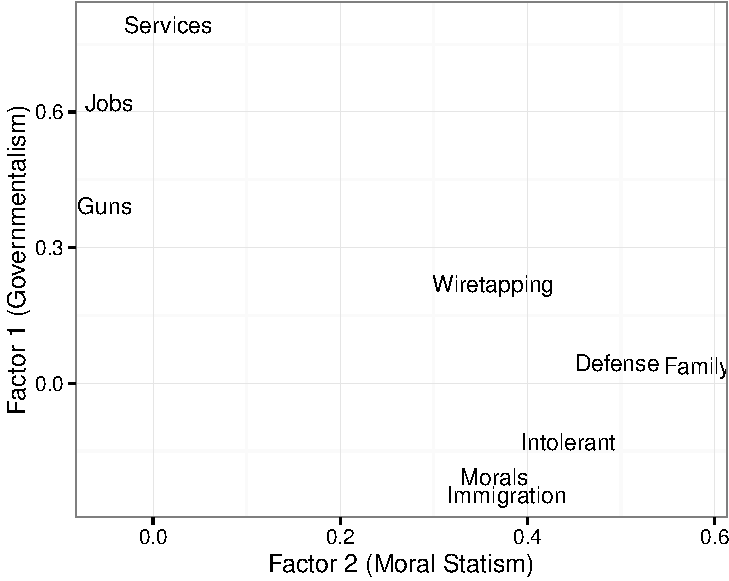
\includegraphics{figures/factorplot-1.pdf}
\caption{Factor plot shows two main dimensions}
\end{figure}

\pagebreak

\singlespacing

\begin{table}[!htbp] \centering 
  \caption{Logistic Regressions, Tea Party Support} 
  \label{} 
\footnotesize 
\begin{tabular}{@{\extracolsep{5pt}}lcc} 
\\[-1.8ex]\hline 
\hline \\[-1.8ex] 
\\[-1.8ex] & (1) & (2)\\ 
\hline \\[-1.8ex] 
 Gender (Male) & 0.238$^{*}$ & 0.128 \\ 
  & (0.124) & (0.128) \\ 
  Income & $-$0.176 & $-$0.323$^{**}$ \\ 
  & (0.142) & (0.147) \\ 
  Conservatism & 1.350$^{***}$ &  \\ 
  & (0.192) &  \\ 
  Age & $-$0.246$^{*}$ & $-$0.379$^{***}$ \\ 
  & (0.138) & (0.144) \\ 
  Race (White) & $-$0.338$^{**}$ & $-$0.451$^{***}$ \\ 
  & (0.162) & (0.167) \\ 
  Education & 0.114 & 0.059 \\ 
  & (0.153) & (0.159) \\ 
  Obama & $-$1.820$^{***}$ & $-$1.300$^{***}$ \\ 
  & (0.200) & (0.223) \\ 
  Authoritarianism & 0.028 & 0.030 \\ 
  & (0.142) & (0.147) \\ 
  BornAgain & 0.370$^{***}$ & 0.287$^{**}$ \\ 
  & (0.131) & (0.135) \\ 
  Religion & $-$0.040 & $-$0.016 \\ 
  & (0.152) & (0.155) \\ 
  PartyID (Republican) & 0.357$^{*}$ & 0.431$^{**}$ \\ 
  & (0.194) & (0.198) \\ 
  FoxNews & 0.776$^{***}$ & 0.696$^{***}$ \\ 
  & (0.130) & (0.133) \\ 
  MoralStatism &  & 0.671$^{**}$ \\ 
  &  & (0.281) \\ 
  Government &  & $-$0.756$^{***}$ \\ 
  &  & (0.264) \\ 
  MoralStatism*Government &  & $-$1.450$^{***}$ \\ 
  &  & (0.320) \\ 
  Constant & $-$2.600$^{***}$ & $-$2.540$^{***}$ \\ 
  & (0.202) & (0.207) \\ 
 \hline \\[-1.8ex] 
Observations & 2,406 & 2,406 \\ 
Log Likelihood & $-$856.000 & $-$833.000 \\ 
Akaike Inf. Crit. & 1,738.000 & 1,695.000 \\ 
\hline 
\hline \\[-1.8ex] 
\textit{Note:}  & \multicolumn{2}{r}{$^{*}$p$<$0.1; $^{**}$p$<$0.05; $^{***}$p$<$0.01} \\ 
\end{tabular} 
\end{table}

\pagebreak

\doublespacing

\begin{figure}[htbp]
\centering
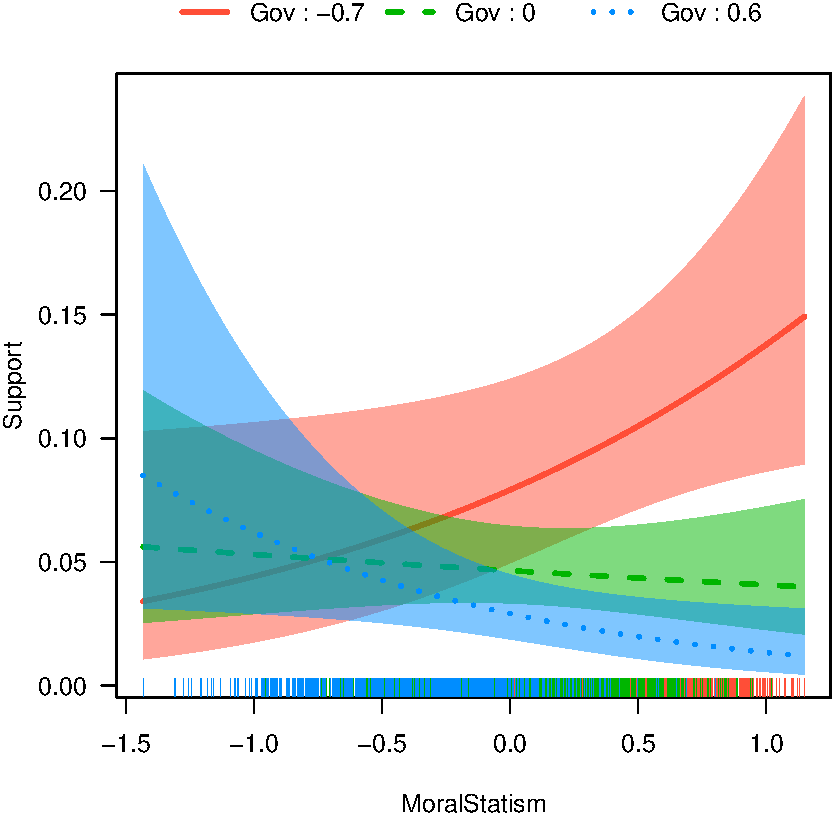
\includegraphics{figures/effect-plot1-1.pdf}
\caption{The Effect of Moral Statism Conditional on Govermentalism
(Gov)}
\end{figure}

\end{document}